%! Author = mumoe
%! Date = 4/13/2022

\documentclass[../main.tex]{subfiles}


\begin{document}

\onehalfspacing

%-------------------------------------------------------------------------
%----------------------------------REDES----------------------------------
%-------------------------------------------------------------------------


En este capítulo, se mostrarán los fundamentos teóricos utilizados en este trabajo. Se comienza con teoría de redes y termina hasta una síntesis de la entropía de Shannon.

\section{Teoría de Redes.}
%Es un breve resumen sobre redes (inlcuir a Euler, Moreno, Milgram, Strogatz, Babarbasi)

% A continuación, se presentará un contexto histórico del desarrollo de la teoría de redes.


El problema de los puentes de Königsberg resulta ser la motivación pionera en la teoría de gráficas. La  ciudad de Königsberg fue fundada por los caballeros teutónicos en el año 1255 y, debido a su asentamiento sobre el río Pregolia, se convirtió en un importante centro de intercambio. Debido al desarrollo del río Pregolia, este dividió a la ciudad en cuatro regiones conectadas por siete puentes (ver figura \ref{fig:marcoteorico_konigsberg}).



\begin{figure}[h!]
    \centering
    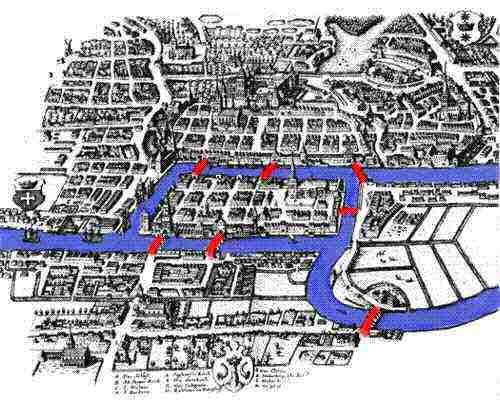
\includegraphics[scale = 0.5]{images/marcoteorico_konigsberg.jpg}
    \caption{Una vista de Königsberg mostrando en rojo los siete puentes sobre el río Pregolia.  }
    \label{fig:marcoteorico_konigsberg}
\end{figure}

Al contrario del avance posterior de la Matemática, resulta que este problema no es más que un simple análisis de un juego entre los habitantes de Königsberg. El susodicho problema consistió en recorrer cada uno de los puentes una sola vez.

Fue hasta el año 1741 cuando se hace público el artículo de Leonhard Euler dando una solución particular y general a este problema. Lo más esencial de este texto de 21 párrafos es la simplicidad de la solución. Euler propone enfocarnos en las conexiones generadas por los puentes; explícitamente, identificar a cada segmento de tierra con una letra mayúscula y cada puente con una letra minúscula (ver figura \ref{fig:marcoteorico_abstracteuler}).   De esta simplificada representación, se deducen diversos resultados a través de conteos experimentales; siendo que aquí no sólo se da una solución al problema, sino una generalización.

Es curioso mencionar que debido a la sencillez del planteamiento del problema, Euler no cree necesaria la intervención de una visión matemática al mismo \cite{thetrueaboutkonigsberg}. Este artículo motivó al enfoque de los problemas en una abstracción de objetos y sus relaciones. Con ello, el inicio de una rama más de la Matemática: Teoría de Gráficas.



\begin{figure}[h!]
    \centering
    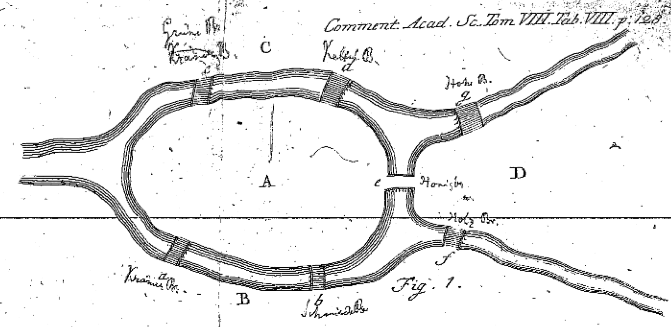
\includegraphics[scale = 0.5]{images/marcoteorico_abstract.png}
    \caption{Esbozo original de Euler sobre el problema de los puentes de Königsberg.}
    \label{fig:marcoteorico_abstracteuler}
\end{figure}


%Dejemos pendiente Jacobo Levy Moreno
%Some ideas:
%-Breve descripción de socioMETRÍA.
%Metemos a Jacabo con alguna aportación importante.

Una abstracción intuitiva para un pensamiento actual es extrapolar estos hacia las relaciones humanas, algo innovador para el pensamiento del siglo XIX. Jacobo Levy Moreno, influenciado por diversas culturas y diferencias sociales, pronto comenzó a considerar la afinidad y preferencia de la gente por relacionarse ante distintas adversidades \cite{moreno_intro}. Esta sencilla observación dio origen a la sociometría que fue impulsada por los sociogramas, represenataciones gráficas de relaciones sociales, hechos por Jacobo Moreno.

%Standley Milgran; principios del Mundo pequeño.

Siguiendo la línea del análisis del comportamiento social, en 1967, Stanley Milgram induce una pregunta a través situaciones cotidianas asociada al fenómeno de \textit{mundo pequeño}: cualquiera dos personas en el mundo están a pocas personas de conocerse. La pregunta que planteada es sencilla: ¿cuantas conexiones entre dos personas son necesarias para que estas se conozcan? El problema y solución recae en la estructura matemática de la sociedad \cite{milgram1967small}. La parte experimental de este proceso concluyó que la cantidad de personas intermedias es apenas un poco más de cinco personas \cite{milgram1967small}.


No fue sino hasta finales del siglo XX que se comienza una formalización de las observaciones antes vistas. En 1998, Duncan Watts  y  Steven Strogatz, a través de un modelo que itera probabilísticamente las aristas de una red regular se encontró una dinámica interesante en función de la estructura topológica de la red \cite{Watts1998}. En específico, se mostró un umbral donde la red tiene un coeficiente de agrupamiento lo suficientemente alto pero con una distancia media entre los nodos corta.  Si bien esta conclusión de la propiedad de mundo pequeño nunca fue definitiva, sí indujo diversas incertidumbres y otras formalizaciones de las mismas; aunque, muchas son en función de lo mostrado por Watts y Strogatz \cite{Telesford2011}.


A partir de la motivación de Watts y Strogatz, el desarrollo complementario de Barabasi al mundo de los sistemas complejos fomentó aun más la investigación en redes. En 1999, poco después de la publicación de Watts y Strogatz, Albert-László Barabási y Réka Albert analizaron la red de citas de páginas de internet. De esto, el aspecto más relevante es inducir una nueva dinámica en redes desde un paradigma distinto a la aleatoridad: Las \textit{redes de libre escala} \cite{Barabasi1999}. Este tipo de red presenta una propiedad interesante en su distribución de grado, pues se distribuye como una ley de potencia; de manera formal, si $f(x)$ es la distribución de grado, entonces es $f$ es ley de potencia si $f(x) \sim x^{-\alpha} $ con $\alpha > 0$. Esta caracterización de la distribución de grado induce a que la red en cuestión contenga \textit{hubs} (nodos con un grado muy alto).  Esto último consecuencia de dos propiedades relevantes: el continuo nacimiento de nuevos enlaces y la preferencia de relacionarse a un nodo en particular \cite{Barabsi2005}.


\begin{figure}[h!]
    \centering
    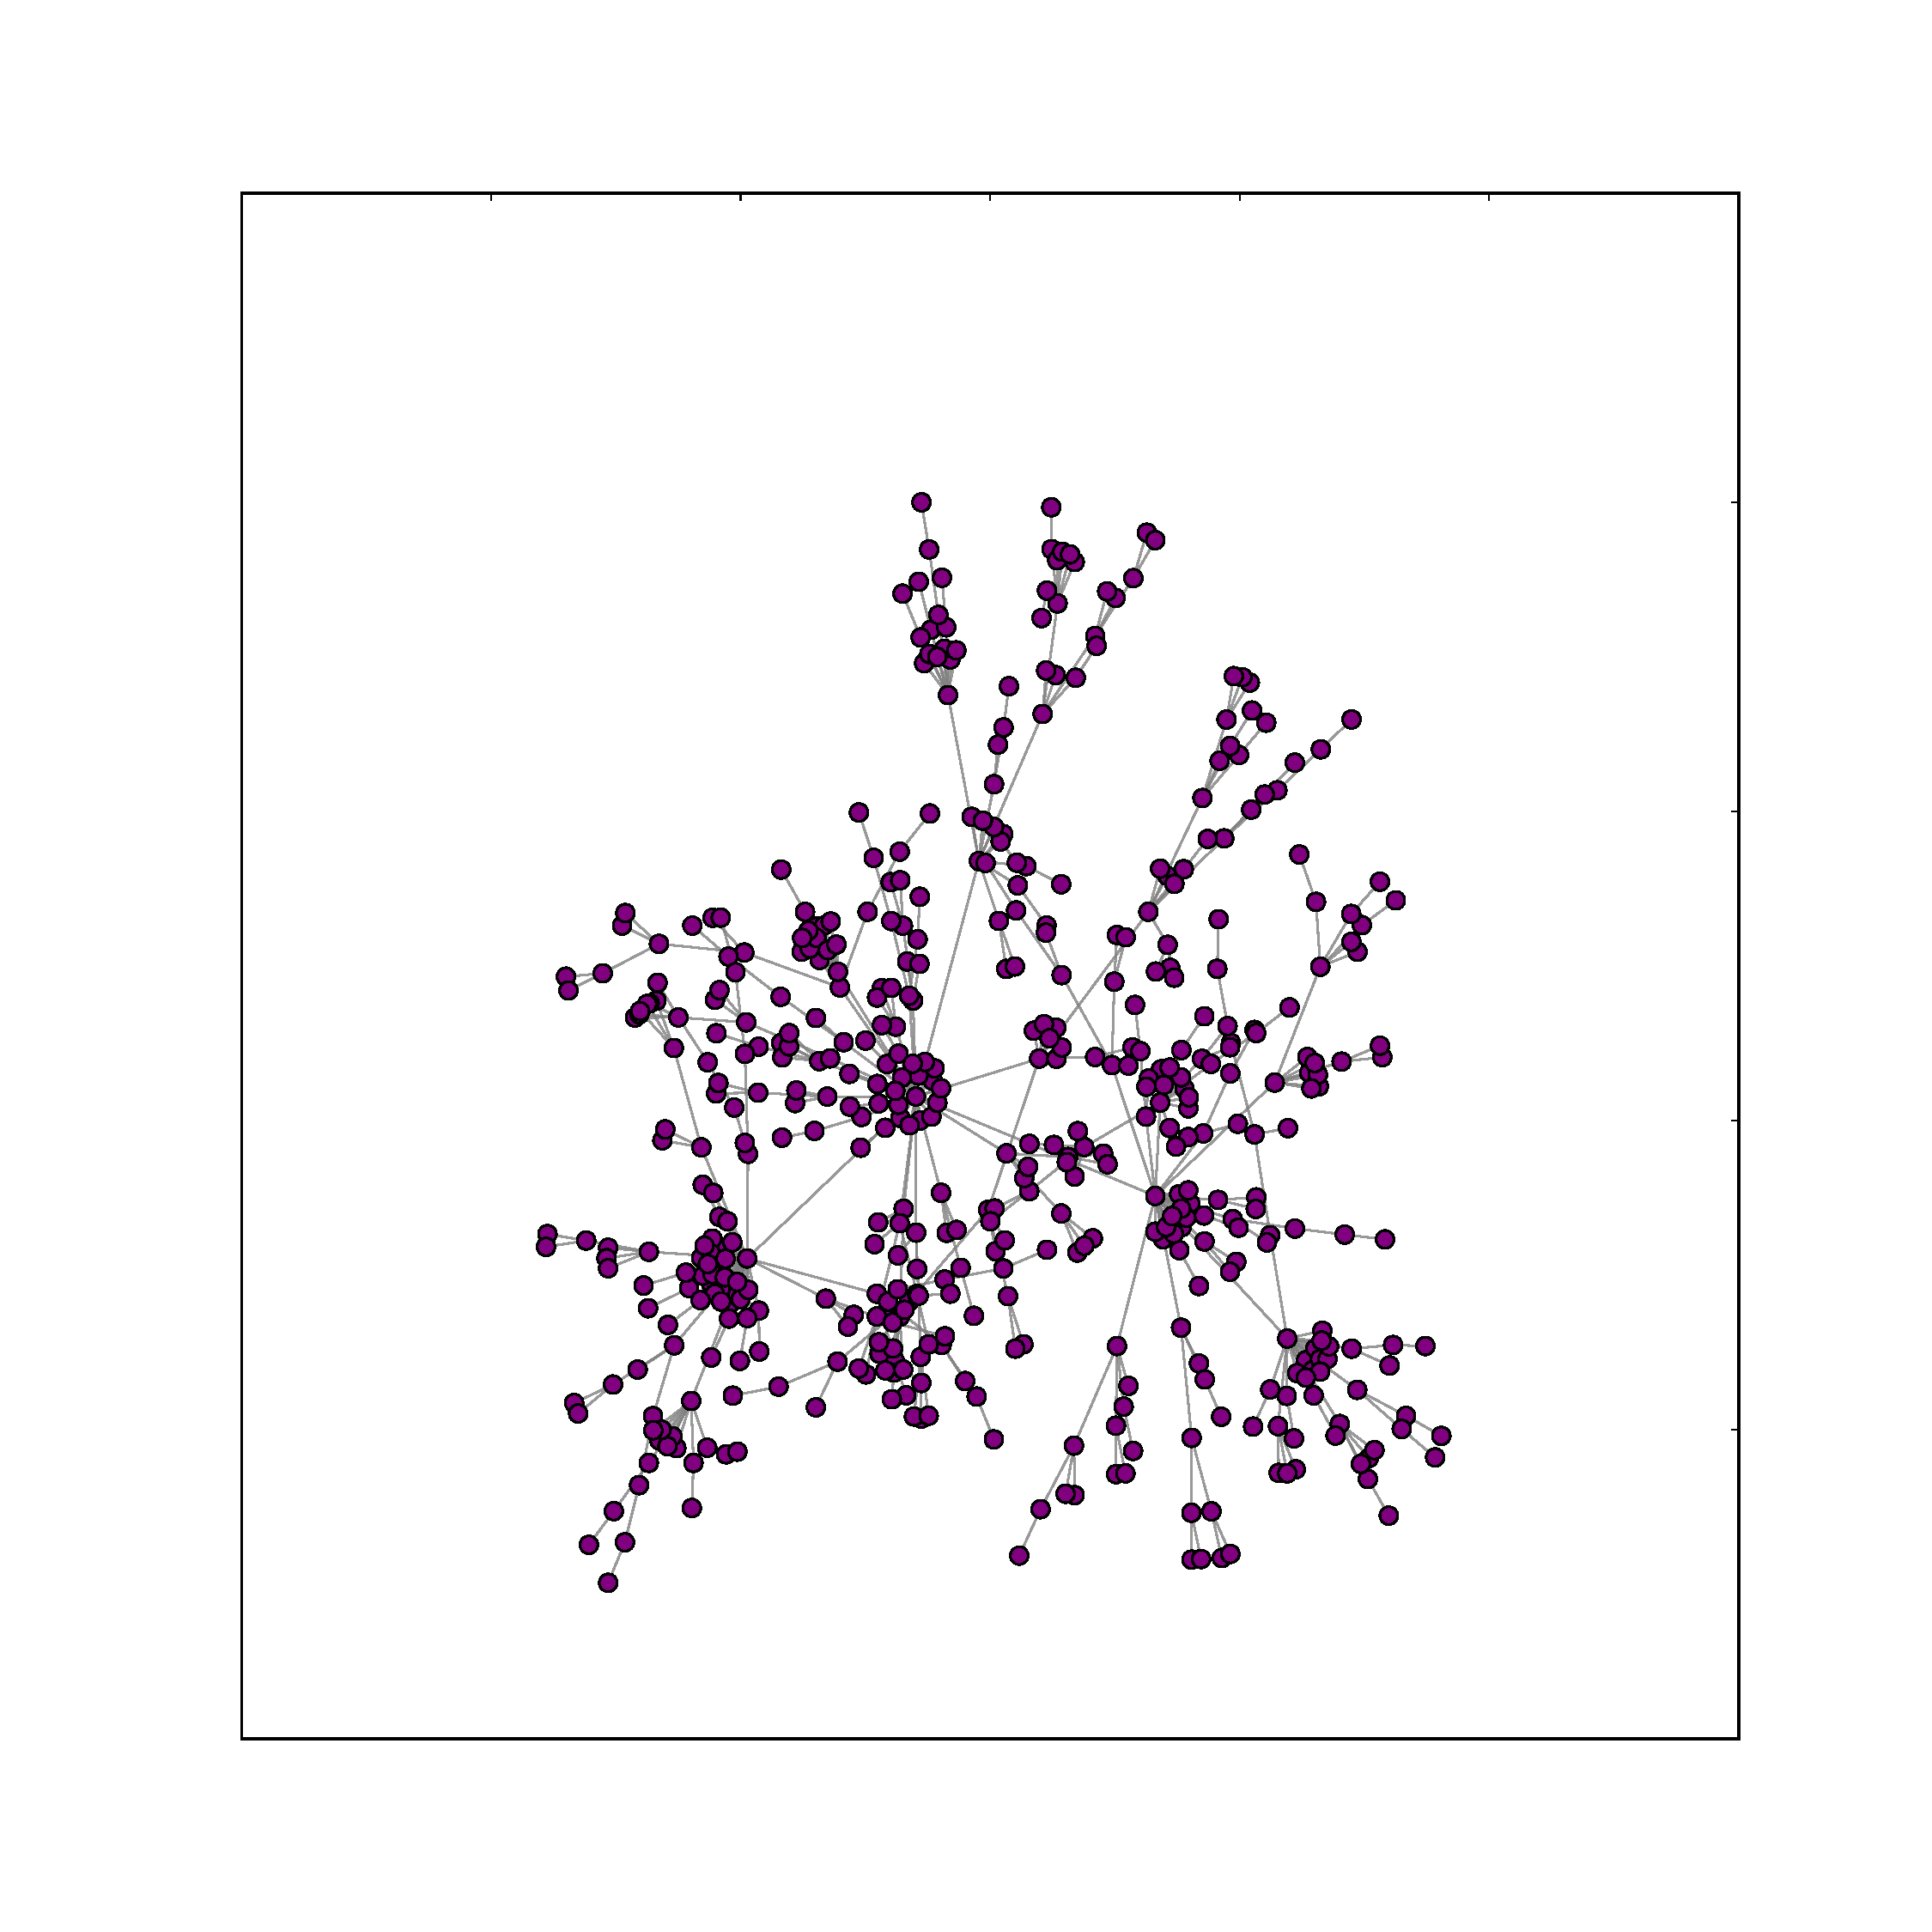
\includegraphics[scale = 0.35]{images/marcoteorico_barabasi.pdf}
    \caption{Ejemplo de una red de libre escala. Fuente: Elaboración propia.}
    \label{fig:marcoteorico_scale_free}
\end{figure}

%Como lo mencionan Strogatz


% \begin{figure}
% \centering
% \begin{minipage}{.5\textwidth}
%   \centering
%   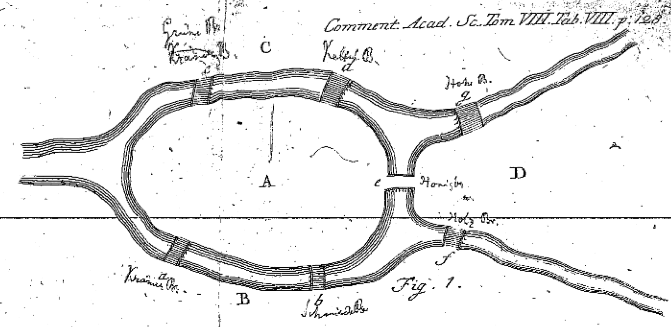
\includegraphics[width=.4\linewidth]{images/marcoteorico_abstract.png}
%   \captionof{figure}{A figure}
%   \label{fig:test1}
% \end{minipage}%
% \begin{minipage}{.5\textwidth}
%   \centering
%   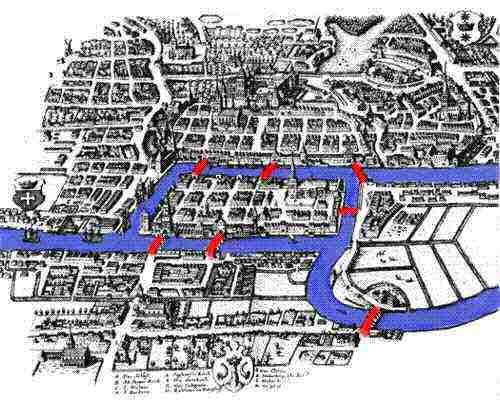
\includegraphics[width=.4\linewidth]{images/marcoteorico_konigsberg.jpg}
%   \captionof{figure}{Another figure}
%   \label{fig:test2}
% \end{minipage}
% \end{figure}

\newpage
\subsection{Definiciones de Teoría de Redes.}

%Definimos una red en general.
En esta sección se presentarán las definiciones formales de una red y sus métricas. En lo que del texto, se define a $V$ como un conjunto de nodos y a $E$ como un conjunto de aristas.

\subsubsection{Red no dirigida y dirigida.}


Una red  es una gráfica o pareja ordenada $G = (V,E)$, que tiene una interpretación. Esta interpretación dependerá del sistema en cuestión a investigar.

La distinción entre una red dirigida y una red no dirigida es la forma en la cual se define el conjunto $E$. Por una lado, una \textit{red no dirigida} no nos importan el orden de los enlaces. Por el otro lado,una \textit{red dirigida} sí.



\begin{figure}[h!]
    \centering
    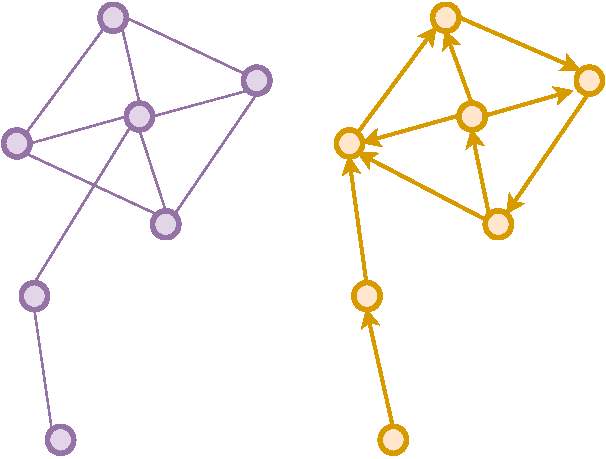
\includegraphics[scale = 0.8]{images/marcoteorico_graphdigraph.pdf}
    \caption{Ejemplos de una red dirigida y no dirigida. De lado izquierdo tenemos una red no dirigida. De lado derecho, una red dirigida. }
    \label{fig:marcoteorico_graph_digraph}
\end{figure}

\subsection{Red temporal.}

Una principal característica de las redes dirigidas y no dirigidas es que ambas son estáticas : una vez que la relación se haya definido, no va a cambiar. Así, esta forma de modelación tiene una implicación en definir la relación de los entes del sistema como relaciones binarias.

Una red temporal se puede definir como una composición de redes no dirigidas (o dirigidas) indexadas por tiempo. La definición del índice de tiempo proviene de una secuencia discreta de tiempo.  En palabras generales, no es más que definir cada una de las redes con los nodos o enlaces de interés en el lapso de tiempo fijo. Definamos a $T$ com la longitud del lapso de tiempo. Por ejemplo, este valor de $T$ puede ser una hora o 25 minutos.

De manera formal, definamos $t \in \{ 1, 2, 3, \dots , n_{max} \}$ es la secuencia de discreta de tiempo obtenida. Sea $G_{t} [ V_{t} , E_{t}] $ la red de interés con nodos $V_{t}$ y enlaces $E_{t}$. Entonces, la \textit{red temporal} se puede definir como

\begin{equation*}
    \mathcal{G} = \{ G_{t} \}_{t = 1 }^{n_{max} }
\end{equation*}

La red temporal no es más que una sucesión de redes en específicos que nos los nodos nos están relacionados entre capas.  Una pequeña ilustración de esta red en particular se puede ver en la gráfica \ref{fig:marcoteorico_redtemporal}.

\begin{figure}[h!]
    \centering
    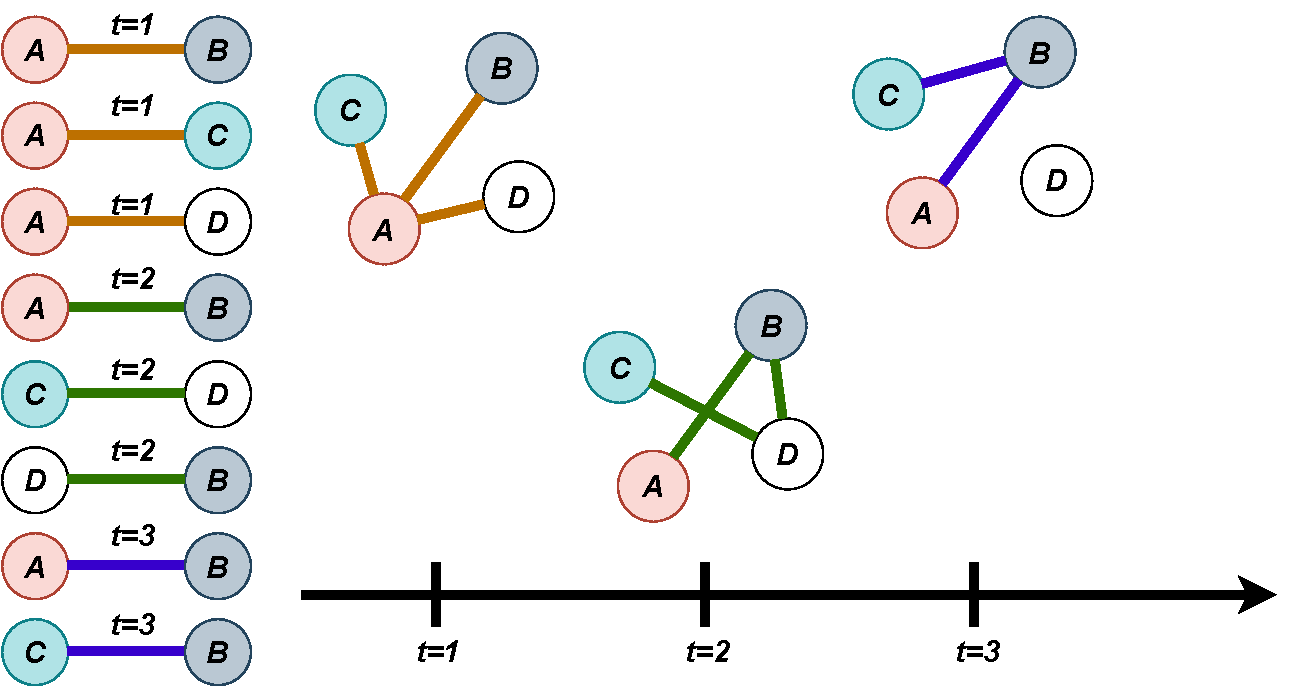
\includegraphics[scale = 0.6]{images/marcoteorico_redtemporal.drawio.pdf}
    \caption{Representación de una red temporal. Se observa como el enlace $(A,B)$ fue estable en toda la dinámica. }
    \label{fig:marcoteorico_redtemporal}
\end{figure}


% PROPONER UNA NUEVA LINEA DONDE VEAMOS LA COMPARACIÓN ENTRE MÉTRICAS.
% AQUÍ SE PUEDE USAR LA IMAGEN COMPARTATIVA

%Considerar un red temporal
% \subsection{Red inducida por nodos.}




%-------------------------------------------------------------------------
%----------------------------------MÉTRICAS----------------------------------
%-------------------------------------------------------------------------
\subsection{ Métricas.}

En esta sección, se presentan diversas métricas aplicadas en este trabajo. Podemos separarlas por locales (dando la importancia del nodo) y globales (dando la importancia en la topología de la red).

Una de las principales topologías que se toman para el cálculo de las métricas es una noción de distancia entre los nodos. En general, cada una se basa en un tipo particular  de \textit{camino} que hay entre dos nodos. Un camino se define como una sucesión de nodos donde entre cada dos hay un enlace.

\subsubsection{Centralidad intermedia  (\textit{betweenness}) }

Es de suma importancia considerar los múltiples caminos que puede existir entre dos nodos. En particular, es de interés conocer aquellos nodos que juegan un papel relevante ante un tipo de camino: los caminos más cortos. Un camino más corto es aquel donde la longitud es mínima. Nótese que puede existir más de un camino más corto.
Formalmente, esta métrica se representa por

\begin{equation}
    \label{eq:betweennes}
    B(v) = \sum_{v \neq j, i \in V} \frac{ \sigma( i,j | v) }{\sigma( i,j)}
\end{equation}

donde $v \in V$, $\sigma(i,j)$ representa el número de caminos más cortos entre los nodos $i$ y$j$; y $\sigma(i,j|v)$ representa el número de caminos más cortos entre los nodos  entre $i$ y $j$ que pasan por $v$.

La interpretación de esta métrica varía del objeto de estudio en cuestión. Sin embargo, en general, su abstracción se denota por su importancia del nodo en la comunicación con los demás.


\subsubsection{Coeficiente de agrupamiento (\textit{clustering}) }

Uno de los primeros patrones que hay en las redes es la aparición del ciclo más pequeño: \textit{triángulos}. Un triángulo es un camino de longitud tres donde el primer nodo es el último. El coeficiente de agrupamiento no es más que un conteo de aquellos triángulos existentes sobre los ideales en una red con todos los enlaces faltantes para completar los triángulos.

De manera formal, dejemos fijo a un nodo $i$. Si $t_{i}$ representa el número de triángulos donde el nodo $i$ es parte de éste y $d_{i}$ es el grado del nodo. Entonces, su coeficiente de agrupamiento es

\begin{equation}
    \label{marcoteorico_clustering}
    C_{i} = \frac{ t_{i} }{ \frac{d_{i} (d_{i} - 1 )}{ 2 }} = \frac{2 t_{i} }{d_{i} (d_{i} - 1 ) }
\end{equation}

Notemos que, el denominador de la expresión es el número de triángulos posibles entre sus vecinos. De la propia definición, es positiva y el valor máximo es 1.




\subsubsection{Coeficiente de cercanía (\textit{closeness}) }

Es el coeficiente de cercanía de un nodo hacia los demás nodos. En ese sentido, valores altos en esta métrica simbolizan un sentido de centralidad en la red.

De manera formal, si $d(u,v)$ representa la longitud del camino más corto entre $u$ y $v$: y $n$ es la cardinalidad del conjunto $V$. Entonces, el coeficiente de cercanía de un nodo $u$ es

\begin{equation}
    \label{marcoteorico_closeness}
    close(u) = \left(\frac{\sum_{v \neq u} d(u,v) }{n-1} \right) ^{-1}
\end{equation}


\subsubsection{Centralidad $k-\text{núcleo}$ (\textit{k-core}) }

Esta métrica de centralidad, al contrario de enfocarnos sobre caminos más cortos, se interesa por el grado propio del nodo.

De manera formal, particiona a cada uno de los nodos con el grado que estos tengas. Podemos ver a $V = \bigcup_{i=1}^{k} D_i $, donde $k$ es el grado máximo y $D_{i} = \{ v \in V | \text{máximo grado de $v$ es } i \}$

\begin{figure}
    \centering
    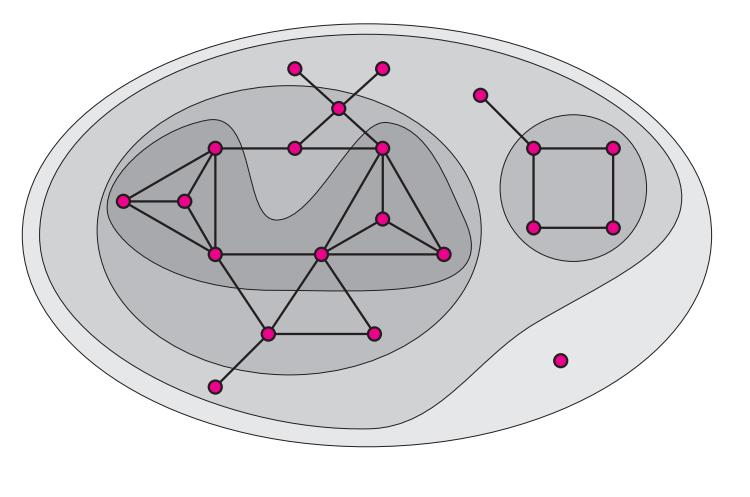
\includegraphics[scale = 0.5]{images/marcoteorico_kcore.png}
    \caption{Ejemplo de la aplicación de la métrica $k-\text{núcleo}$. (Fuente:  \cite{DBLP:journals/corr/cs-DS-0310049}.}
    \label{fig:my_label})
\end{figure}




% \subsubsection{Centralidad de Katz}

% El grado de un nodo en la red es una de las  primeras métricas para  importancia del mismo. En un caso muy puntual, a cuantos
% % Katz (katz), es el coeficiente de centralidad similar
% % al eigenvector ; este valor ser ́a mayor cuanto m ́as est ́e
% % conectado a los dem ́as nodos aunque su aportaci ́on
% % cada vez sea menor.

\subsubsection{Centralidad de vector propio (\textit{eigenvector}) }

La caracterización de un nodo puede ser definida por sus vecinos inmediatos; eres por quienes te juntas y tienes mayor contacto. Esta noción la recupera esta métrica. El cálculo de la misma es resolver una operación matricial:

\begin{equation}
    \label{marcoteorico_eigenvector}
    A x = \lambda x,
\end{equation}

donde $A$ es la \textit{matriz de adyacencia} de la red y $\lambda > 0 $ es el valor propio más grande de la matriz de adyacencia.  La matriz de adyacencia de una red es una matriz donde las entradas de la misma representan los enlaces entre los nodos; las columnas y renglones son la representación de los nodos. De manera formal, para cualesquiera dos nodos $i,j \in V$, tenemos que:

\begin{align*}
    (A)_{i,j} &= \begin{cases}
1 & \text{ Si } (i,j) \in  E  \\
0 & \text{ En caso contrario.}
\end{cases}
\end{align*}

Esta matriz es útil para otras métricas de interés que requieren conocer las relaciones entre los nodos. En particular, de la expresión \eqref{marcoteorico_eigen} podemos ver como la ponderación de la importancia de tus primeros vecinos sea hace de forma lineal.

\subsubsection{Índice de Katz }

Una problemática con la expresión en \eqref{marcoteorico_eigen} es que sólo involucra a los vecinos en su primera \textit{vecindad} de cada nodo. La n-ésima vecindad de un nodo se define como al conjunto de nodos donde hay un camino de longitud $n$.

El índice de Katz extiende la noción de la influencia de nodos que pertenencen más allá de la primera vecindad. En efecto, el cálculo de la misma pondera su importancia a partir de todos los posibles caminos de longitud $k$ entre los nodos.

\begin{equation}
    \label{marcoteorico_katz}
    Katz(i) &= \left[ \sum_{k = 0}^{\infty} ( \alpha A )^{k} e\right]_{ i }
\end{equation}

dodne $e$ es el vector que en todas las entradas tiene 1. La implementación de considerar todos los caminos de longitud $k$ está llevada a cabo por el producto matricial $A^{k}$. Nótese que, como en la métrica de autovector, la ponderación es lineal debido a la definición de producto matricial.




\begin{figure}[h!]
    \centering
    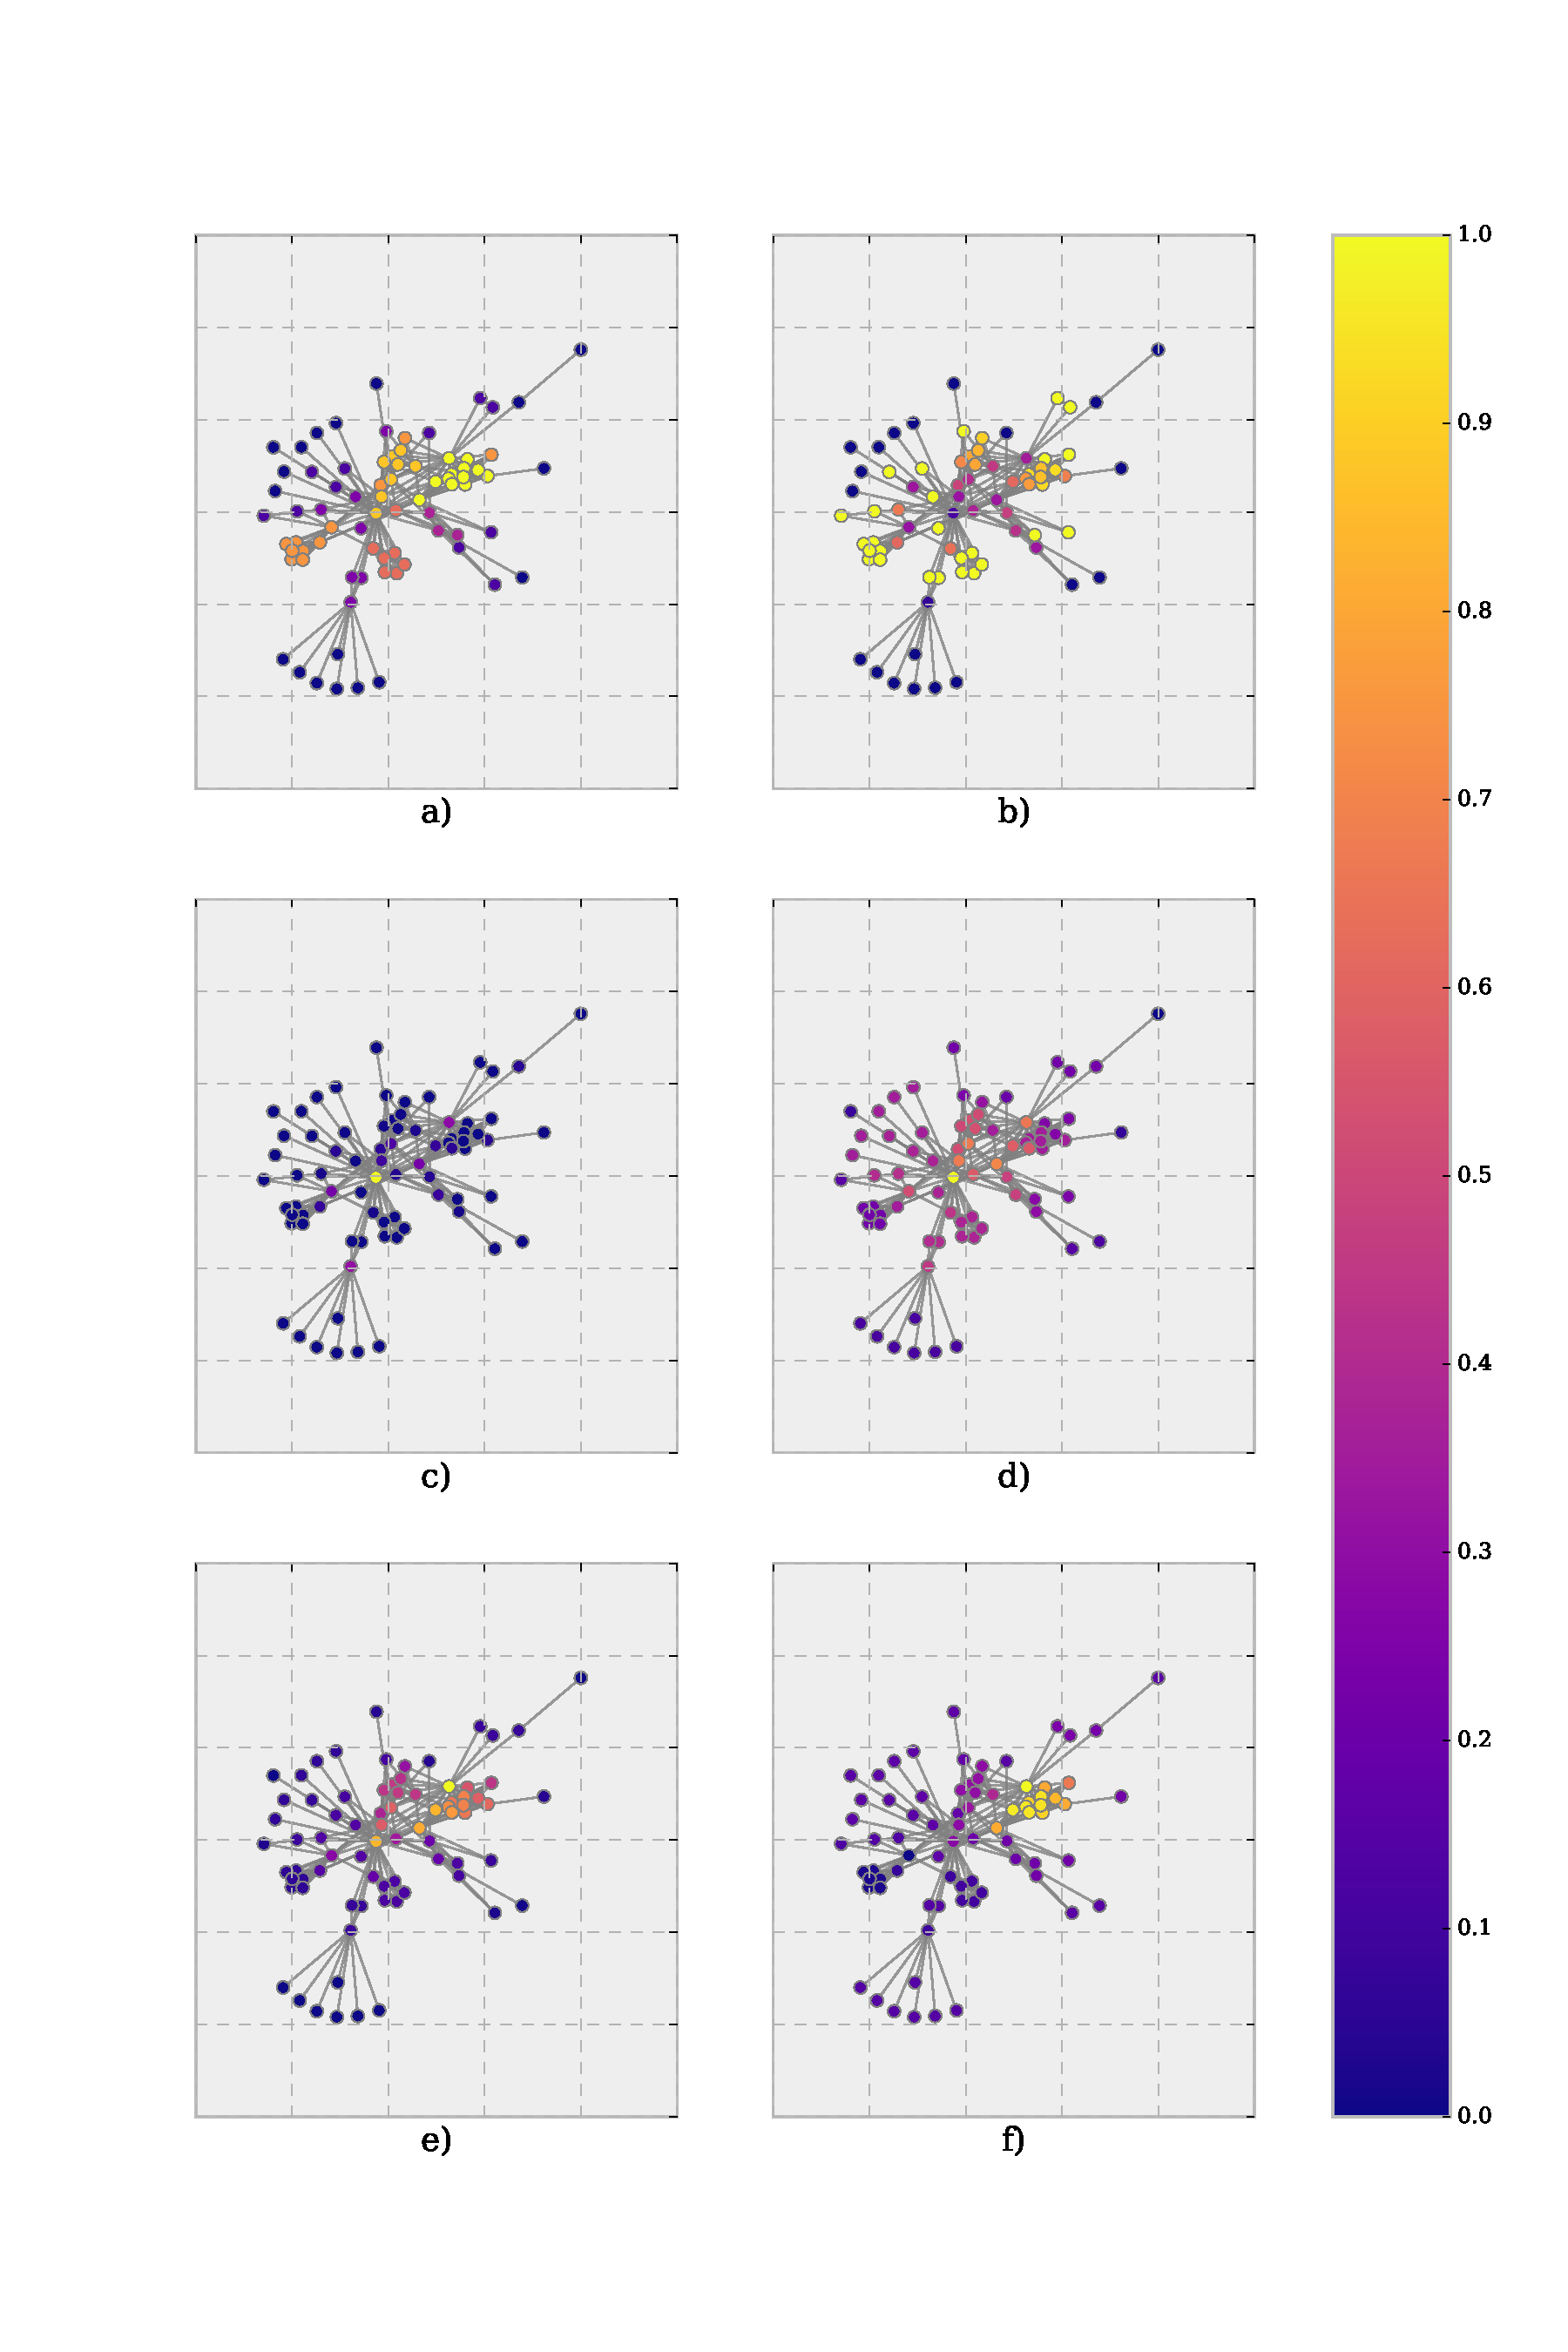
\includegraphics[scale = 0.40]{images/marcoteorico_barabasi (1).pdf}
    \caption{Comparativo de métricas para la red del Karate Club  de Zachary. Las métricas que se muestran son a) k-núcleo, b) clustering, c) betweeness, d) closeness, e) eigenvector y  f) centralidad de Katz.   Fuente: Elaboración propia.}
    \label{fig:marcoteorico_scale_free}
\end{figure}


%-------------------------------------------------------------------------
%----------------------Sistemascomplejos----------------------------------
%-------------------------------------------------------------------------
\section{Sistemas Complejos.}

Los sistemas complejos estudian la forma de los componentes y su interacción entre sí; '\textit{pueden espontáneamente auto-organizarse y presentar
estructuras globales y comportamientos no-triviales a mayores
escalas, sin intervención externa, autoridad central o líderes que
determinen el comportamiento colectivo}' \cite{complejidad_explicada}. Si bien no se puede hablar de una definición formal de los sistemas complejos, sí es posible identificar ciertas características, que a continuación se explican.

\textbf{1. \textit{Sistémica} y \textit{sinérgica}}. Las relaciones o interconexiones en un sistema pueden ser lineales, indicando la propiedad sistémica, sin embargo no significa que sea un sistema complejo, para ello es necesario considerar la propiedad de sinergia. Es decir, las interacciones deben ser no lineales entre las partes de un sistema.


% Si bien esto no es una definición formal, capta la importancia del estudio en estos sistemas: las relaciones.

%%





% Se podría volar
Se han detectado propiedades en común sobre dichos sistemas. Como en el caso de su definición, puede variar dependiendo del autor y el sistema a estudiar. Las propiedades que se consideran más importantes son tres: \textit{emergencia}, \textit{autoorganización} , \textit{independencia} e \textit{interdependencia}.

% Se podría mantener (pero ahorita)
Las últimas dos propiedades muestran la robustez del sistema ante perturbaciones del mismo. En efecto, notaremos que existen relaciones clave en un sistema que, en la ausencia de estas, pueden colapsar todo el sistema. Así mismo, también encontraremos relaciones fuertes que, en la ausencia de estas, el sistema no sufrirá daño.

% Se podría mantener (pero ahorita)
La \textit{autoorganización} y la propiedad emergente destacan por la necesidad de cambio por la estabilidad o beneficio del sistema aún cuando no exista un líder o reglas formalmente escritas o explícitas. Pues, cada componente del sistema puede actuar por su beneficio propio autoorganizándose y, a nivel global, generar un patrón de cambio repentino o un estado emergente.





\newline
\subsection{Entropía de Shannon.}

En teoría de la información se estudia como la información es comprimida o transmitida. De forma ocasional, este estudio se  considera un subconjunto de la teoría de la comunicación \cite{cover2006elements}.

De esta forma, nacen métricas con una intuición sencilla pero aplicaciones complejas. La entropía, en este campo, se define como un promedio de la incertidumbre del verdadero estado de un fenómeno. Para una variable aleatoria $X$, con función de distribución de probabilidad $f(x)$, la entropia de Shannon se define como

\begin{equation}
    \label{shannon-entropy}
    H(X) = - \sum_{x} f(x) \log_{2} ( p(x))
\end{equation}

El valor resultante, para el caso de $\log_{2}$, se llama $bits$ de información.

La interpretación de esta métrica es sencilla: ¿Cuántas preguntas con respuesta binarias se necesitan para saber el estado actual del sistema? Pues, entre mayor número de preguntas se necesiten mayor es la incertidumbre. En consecuencia, cuando $X$ tiene un sesgo para cierto valores, la entropía es baja; ya que, el valor de $X$ es más probable que esté en la parte sesgada.

Notemos que se puede cambiar la base del logaritmo en esta métrica, obteniendo posibles resultados distintos (véase \cite{cover2006elements} para algunas propiedades). En este trabajo, únicamente se usará la entropía de Shannon con logaritmo con base 2.







\end{document}